 \documentclass[letterpaper, titlepage, 11pt]{article}

\usepackage{fullpage}
\usepackage{graphicx}
\usepackage{hyperref}
\usepackage{url}
\usepackage{titling}

% This is here so we can have a fancier title page than LaTeX gives us by default
\newcommand{\department}[1]{%
  \gdef\dept{#1}}
\newcommand{\dept}{}
\renewcommand{\maketitlehookd}{%
\par\noindent \dept }

\title{
	smrt: A 3D Media Center User Interface
	\\
	User's Manual
}
\author{
	Cory Maccarrone  \\ {\small \href{mailto:Cory.Maccarrone@colorado.edu}{Cory.Maccarrone@colorado.edu}}
	\and
	Daniel Seikaly   \\ {\small \href{mailto:Daniel.Seikaly@colorado.edu}{Daniel.Seikaly@colorado.edu}}
	\and
	Evan Sheehan     \\ {\small \href{mailto:Wallace.Sheehan@gmail.com}{Wallace.Sheehan@gmail.com}}
	\and
	David Trowbridge \\ {\small \href{mailto:trowbrds@gmail.com}{trowbrds@gmail.com}}
}
\department{
\begin{center}
	CSCI 4308-4318. Software Engineering Project 1 \& 2 \\
	Department of Computer Science \\
	University of Colorado at Boulder \\
	2005-2006 \\
	\vspace{1.5em}
	Sun Microsystems \\
	Santa Clara, CA \\
	\vspace{1em}
	Paul Byrne \\
	{\small \href{mailto:Paul.Byrne@Sun.COM}{Paul.Byrne@Sun.COM}} \\
	\vspace{1em}
	Hideya Kawahara \\
	{\small \href{mailto:Hideya.Kawahara@Sun.COM}{Hideya.Kawahara@Sun.COM}}
\end{center}
}
\pagestyle{empty}

\begin{document}
\maketitle

\raggedbottom

\pagenumbering{roman}

\hspace{1em}
\pagebreak

\tableofcontents

\pagebreak
\hspace{1em}
\pagebreak

\pagenumbering{arabic}

\documentclass[letterpaper, notitlepage, 11pt]{article}
\usepackage[body={6in, 8in}, left=1in, right=1in, top=1in, bottom=1in]{geometry}
\usepackage{fancyhdr}

\pagestyle{empty}

\begin{document}
\documentclass[letterpaper, notitlepage, 11pt]{article}
\usepackage[body={6in, 8in}, left=1in, right=1in, top=1in, bottom=1in]{geometry}
\usepackage{fancyhdr}

\pagestyle{empty}

\begin{document}
\documentclass[letterpaper, notitlepage, 11pt]{article}
\usepackage[body={6in, 8in}, left=1in, right=1in, top=1in, bottom=1in]{geometry}
\usepackage{fancyhdr}

\pagestyle{empty}

\begin{document}
\input{../lib/project-proposal}
\end{document}

\end{document}

\end{document}


\section{Introduction}
As a company, one of Sun Microsystems' objectives is to innovate the world of
computing. To this end, Sun created Project Looking Glass to explore the field
of 3D user interfaces and determine what improvements in user interaction can be
made by taking advantage of the third dimension. Through Project Looking Glass,
Sun hopes to begin redefining how people think of user interfaces and create
useful design concepts for a 3D computing environment. At the moment, Looking
Glass consists of a framework for developing 3D applications and a desktop
environment to run them alongside existing 2D applications.

The goal of this project, code named \textit{smrt}, is to create a user
interface for a home media center along the lines of TiVo, but using 3D user
interface elements within the Looking Glass environment. The name \textit{smrt}
-- pronounced ``smeert'' -- is the Czech word for ``death,'' and was primarily
chosen because it is fun to say and spell.

Figure \ref{figure:concept} presents a conceptual diagram of the overall
system.  This diagram shows how \textit{smrt} interacts with its software and
hardware environment. At the most basic level, \textit{smrt} allows a user to
browse through and play media, as well as watch or record a TV show.  To control
the system, a simple input device such as keyboard or remote control is used.
Note that this project is focused on the user interface; actual functionality
may not exist.

\begin{figure}[htb]
\centering
\includegraphics[width=4in]{figures/conceptual_overview}
\caption{Conceptual overview of the \textit{smrt} project\label{figure:concept}}
\end{figure}


This document provides step-by-step instructions for setting \textit{smrt} up on
a computer and using it.  Section \ref{sec:install} explains the installation
process; it lists \textit{smrt}'s software dependencies and enumerates the steps
for installing them as well as \textit{smrt}.  \textit{smrt}'s configuration
files are explained in section \ref{sec:config}.  This section provides the
information required to customize \textit{smrt} for a particular media center.
Finally, basic usage is explained in section \ref{sec:use}.

\section{Installation}
\label{sec:install}
This section lists \textit{smrt}'s software dependencies and explains how to
install \textit{smrt}.  The dependencies for building and running \textit{smrt}
are enumerated in section \ref{sec:deps}.  The next section provides
step-by-step instructions for building and starting \textit{smrt}.

\subsection{Dependencies}
\label{sec:deps}
There are two types of dependencies for \textit{smrt}: build and runtime.  The
build dependencies are the pieces of software required to compile \textit{smrt}.
The runtime dependencies are needed in order to run \textit{smrt}.

\subsubsection{Build Dependencies}
\begin{itemize}
\item Sun JDK 1.5
\item Ant
\item Java3D 1.4.0 beta 3 or newer
\item JAI
\item Looking Glas 3D 0.7.1 or newer
\end{itemize}

\subsubsection{Runtime Dependencies}
\begin{itemize}
\item Sun JRE 1.5
\item Java3D 1.4.0 beta 3 or newer
\item JAI
\item X11 window system
\item MPlayer
\item Xine
\item xmltv
\end{itemize}

\subsection{Installing \textit{smrt}}
If you are using a binary build, this section is not applicable.  Please skip to
Section \ref{sec:config}.  To build \textit{smrt}, ensure you have the
dependencies installed, then type \textbf{ant} in the directory with the
\textbf{build.xml} file.

\section{Configuration}
\label{sec:config}
\textit{smrt} allows the user to customize the interface through XML files.
These XML files control the behavior of the menus in \textit{smrt}: they specify
the menu type, menu items, and actions and for the menu items.  The files use
the XML format for serializable objects in Java.  This section explains how to
create these XML files.

\subsection{Configuring Applications}
\label{sec:appconf}
The \textbf{applications.conf} file in the data/ directory is used to select
the applications used for media playback.  The basic format of this file is
XMLBeans.  This file contains one or more application factories and a list of
regular expressions used to identify the file types for which that
application is used.

\begin{verbatim}
<java version="1.5.0" class="java.beans.XMLDecoder">
    <object class="org.jdesktop.lg3d.apps.smrt.application.XineFactory">
        <void property="regexs">
            <array class="java.lang.String">
                <string>.*\.avi/string>
                <string>.*\.mpeg</string>
                <string>dvd\://.*</string>
            </array>
        </void>
    </object>
</java>
\end{verbatim}

The \texttt{XineFactory} class is used to launch Xine, a media player, but any
subclass of \texttt{ApplicationFactory} could be substituted for the
\texttt{class} attribute of the \texttt{object} tag.  Currently, \textit{smrt}
supports MPlayer (\texttt{MPlayerFactory}) and Xine (\texttt{XineFactory}).

\subsection{Configuring Menus}
\textit{smrt}'s menus are completely customizable.  Like application
configuration, menus are configured using XML files.  Each menu has its own XML
file (with the extension \texttt{.menu}) that defines the type of menu and the
items contained in the menu.  Only one of these is actually required: the
\textbf{main.menu} file defines \textit{smrt}'s main menu.  Beyond the main
menu, the user may define as many or as few menus as they like.

\begin{verbatim}
<java version="1.5.0" class="java.beans.XMLDecoder">
    <object class="org.jdesktop.lg3d.apps.smrt.menu.RingMenu"/>
    <object class="org.jdesktop.lg3d.apps.smrt.menu.IconItem">
        ...
    </object>
    <object class="org.jdesktop.lg3d.apps.smrt.menu.IconItem">
        ...
    </object>
    ...
</java>
\end{verbatim}

The first \texttt{object} tag creates the menu, it can be any class that
subclasses \textit{smrt}'s \texttt{Menu} class.  The subsequent \texttt{object}
tags populate the menu with items; each of these must instantiate a subclass of
\textit{smrt}'s \texttt{Item} class.  \textit{smrt} supports three menus that
are populated manually in this fashion: \texttt{RingMenu}, \texttt{ArcMenu}, and
\texttt{CityScape}.

The \texttt{IconItem} class can be used to create items in a ring or arc menu.
It takes five pieces of information in the configuration file: a path to an
image file, an aspect ratio to display the icon, a string to display below the
icon, an action, and an action argument.

\begin{verbatim}
...
<object class="org.jdesktop.lg3d.apps.smrt.men.IconItem">
    <void property="iconFilename">
        <string>home/filePath/tvImage.png</string>
    </void>
    <void property="iconAspect">
        <float>1.0</float>
    </void>
    <void property="label">
        <string>Watch TV</string>
    </void>
    <void property="action">
        <string>push</string>
    </void>
    <void property="actionArgument">
        <string>tv</string>
    </void>
</object>
...
\end{verbatim}

The \texttt{iconFilename} tells the menu item what image to display as the icon;
\texttt{iconAspect} defines the aspect ration at which the image is displayed --
this will most likely be 1.0.  The \texttt{label} property is a string displayed
below the icon in the menu.  The \texttt{action} and \texttt{actionArgument}
properties define the behavior of the menu item when activated.  There are two
actions available to a menu item: ``push'' and ``launch''.  The ``push'' action
causes \textit{smrt} to load a new menu; the menu file that is loaded is
specified as the \texttt{actionArgument} to the ``push'' action.  In the above
example, activating the menu item causes \textit{smrt} to load the menu defined
in the file \textbf{tv.menu} -- note that the ``.menu'' extension is omitted
from the \texttt{actionArgument} string.  The other available action,
``launch,'' launches an application.  The string provided in the
\texttt{actionArgument} is used to determine what application to launch and then
provided as an argument to that application.  For example:

\begin{verbatim}
...
<void property="action">
    <string>launch</string>
</void>
<void property="actionArgument">
    <string>dvd://</string>
</void>
...
\end{verbatim}

\textit{smrt} takes the \texttt{actionArgument} ``dvd://'' and
uses it to find an application configured for that file type (see section
\ref{sec:appconf}).  If it finds one, it then launches that application with
``dvd://'' as an argument.

There are two menus available in \textit{smrt} that do not allow configuration
of items in the fashion just described: the \texttt{TvArcMenu} and the
\texttt{FileSystemCity}.  Both of these menus are special case menus.  The
\texttt{TvArcMenu} is used for navigating TV channels, and the
\texttt{FileSystemCity} is used for file browsing.

The \texttt{TvArcMenu} configuration requires only one piece of information
\textit{viz.} the path to a file that contains channel and program information
in the xmltv format.

\begin{verbatim}
<java version="1.5.0" class="java.beans.XMLDecoder">
    <object class="org.jdesktop.lg3d.apps.smrt.menu.TvArcMenu">
        <string>data/tv.xml</string>
    </object>
</java>
\end{verbatim}

This brief configuration tells \textit{smrt} to create a \texttt{TvArcMenu} and
use the file \textbf{data/tv.xml} as the file containing the programming
information.  It is recommended that the user set up a cron job to update the
data in this file periodically.

Configuring the \texttt{FileSystemCity} is only slightly more complicated.  It
requires a title and a path, and optionally allows you to specify file filters.

\begin{verbatim}
<java version="1.5.0" class="java.beans.XMLDecoder">
    <object class="org.jdesktop.lg3d.apps.smrt.menu.FilesystemCity">
        <void property="title">
            <string>Music</string>
        </void>
        <void property="path">
            <string>/tmp/media/music</string>
        </void>
        <void property="exclusionFilter">
            <object class="org.jdesktop.lg3d.apps.smrt.file.filter.DotFileExclusion"/>
        </void>
        <void property="filenameFilter">
            <object class="org.jdesktop.lg3d.apps.smrt.file.filter.PrettyPrint"/>
        </void>
    </object>
</java>
\end{verbatim}

The ``title'' property is simply used to name the menu; because you may have
multiple \texttt{FileSystemCity} menus -- e.g. one for music, one for video,
etc. -- the title helps to tell them apart.  The ``path'' property tells the
menu what directory to display first. This acts as a root directory, you cannot
traverse below this directory in the menu.  The ``exclusionFilter'' specifies a
class used to prevent the menu from displaying certain files.  And the
``filenameFilter'' is used to manipulate the names of files being displayed.

There are three types of exclusion filters available:
\texttt{DotFileExclusion}, \texttt{ExtensionExclusion}, and
\texttt{CompositeExclusion}.  \texttt{DotFileExclusion} filters out hidden
files (files whose names are prefaced with a ``.'') in the directory.
\texttt{ExtensionExclusion} filters files based on their file extensions.  You
can combine these filters using the \texttt{CompositeExclusion} filter.  For
example, to configure the exclusion filters for a music directory, we might
want to ignore video and image files as well as hidden files.

\begin{verbatim}
<void property="exclusionFilter">
    <object class="org.jdesktop.lg3d.apps.smrt.file.filter.CompositeFilter">
        <array class="org.jdesktop.lg3d.apps.smrt.ExclusionFilter">
            <object class="org.jdesktop.lg3d.apps.smrt.file.filter.DotFileExclusion"/>
            <object class="org.jdesktop.lg3d.apps.smrt.file.filter.ExtensionExclusion">
                <array class="java.lang.String">
                    <string>avi</string>
                    <string>mpeg</string>
                    <string>png</string>
                    <string>jpeg</string>
                </array>
            </object>
        </array>
    </object>
</void>
\end{verbatim}

The file name filter acts on files that have been accepted by the exclusion
filters.  The only available filter at this time is \texttt{PrettyPrint}, which
is used to make the file names nicer for display.  \texttt{PrettyPrint}
replaces underscores with spaces and capitalizes the first letter of each word.
For instance ``03\_moonage\_daydream.mp3'' becomes ``03 Moonage Daydream.mp3''
after passing through the \texttt{PrettyPrint} filter.
  
\section{Use}
\label{sec:use}

Using \textit{smrt} is fairly straight forward.  It has been designed with the
intent of being controlled from a 6-button remote control --- four directional
keys, a `menu' button, and a `select' button.  Everything in \textit{smrt} can be
activated using these six buttons.  This section details the various UI elements
and how to make use of them.

\subsection{General Interaction}
All of the menus and screens in \textit{smrt} have the same general interaction
principles.  Menu items can be selected by using the `select' button.  Items
can be navigated through using the directional buttons.  The `menu' button can
be used to exit from menus.

As menus are traversed, the most recent menu selected is always the one on the
screen.  When exiting a menu, this menu will disappear, replaced with the
previously selected menu.  The highest-level menu, the main menu, cannot be
exited from.

% Should there be more here?

\subsection{Ring Menu}
\label{sec:ring_menu}

\begin{figure}[htb]
\centering
\includegraphics[width=3in]{figures/circle_menu_1}
\caption{A ring menu\label{fig:ring}}
\end{figure}

In \textit{smrt}'s default configuration, the ring menu is the first menu that
is presented upon startup.  It displays the various categories of media available
for play, such as live TV, music, movies, and possibly video game systems.  The
menu can be navigated using the left and right direction buttons to rotate the
menu around.  The selected item is closest to the screen (largest and in center).
An item can be selected by pressing the `select' button.

\subsection{Arc Menu}
\label{sec:arc_menu}

\begin{figure}[htb]
\centering
\includegraphics[width=3in]{figures/arc_menu}
\caption{An arc menu\label{fig:arc}}
\end{figure}

The arc menu is another kind of menu that the user may be presented with.  It is
typically associated with navigation through television channels in choosing a
channel to watch.  The menu is similar to the ring menu, except that navigation
is done using the up and down directional buttons.  The menu does not wrap around
in a ring, but instead ends at the top and bottom.  The selected item is always
centered and can be activated using the `select' button.

\subsection{Cityscape Menu}
\label{sec:cityscape_menu}

\begin{figure}[htb]
\centering
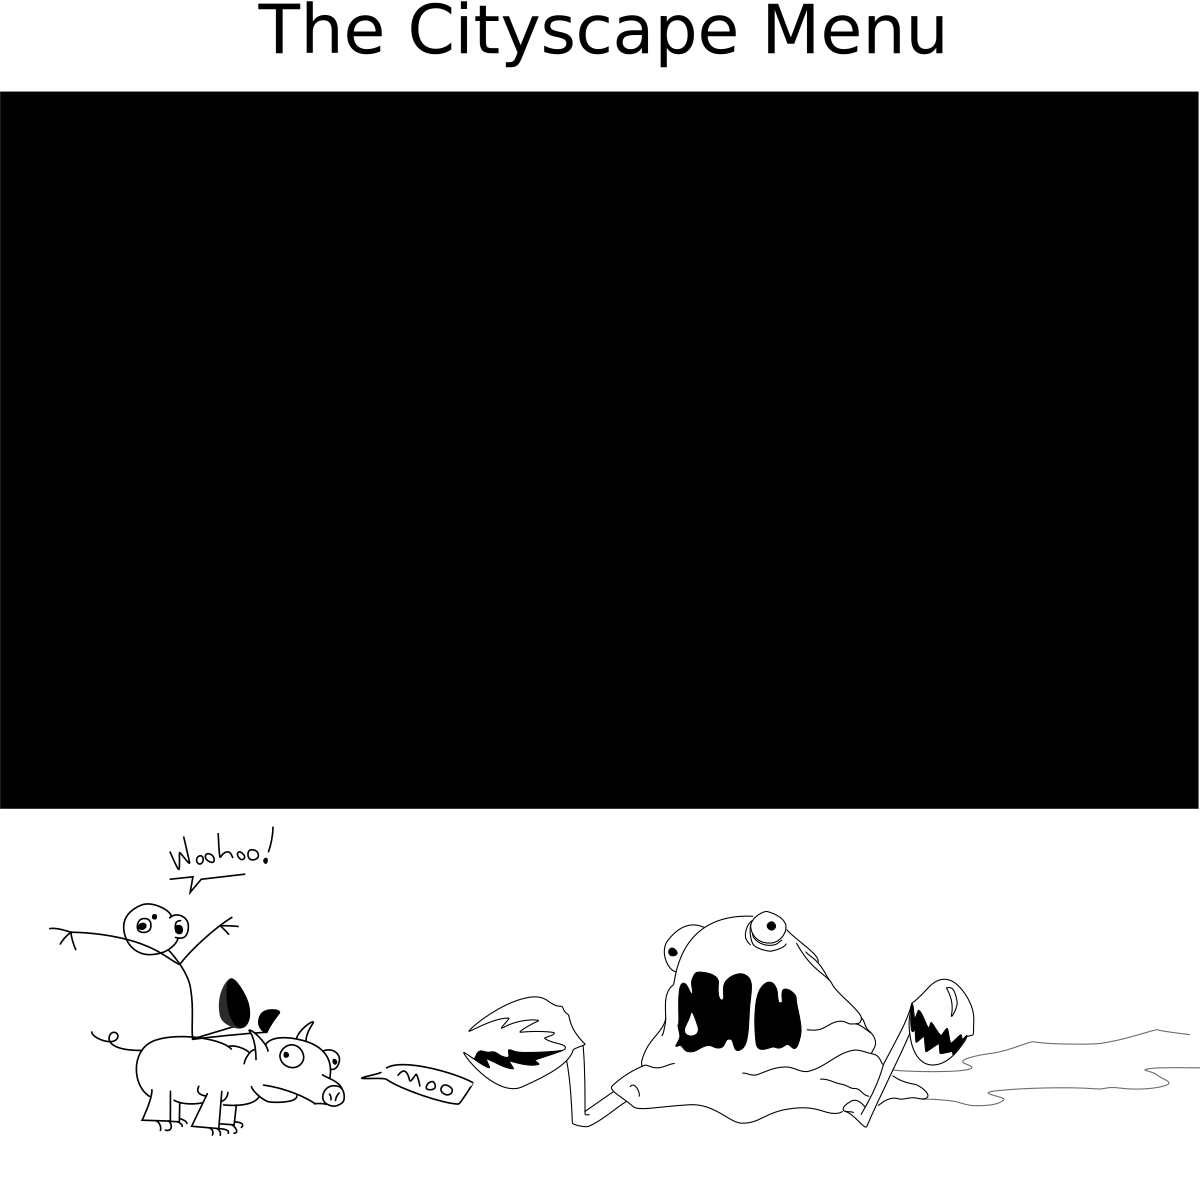
\includegraphics[width=3in]{figures/cityscape}
\caption{A cityscape menu\label{fig:cityscape}}
\end{figure}

The cityscape menu can be used for browsing media of different types --- music,
movies, or videos --- or for anything that would require a large number of items
be presented to the user.  It allows for possibly hundreds of items to choose from.
Each item is represented as a building.  Red buildings are media files.  This
could be an individual song, movie, or video.  Blue buildings represent sub-folders.
These could be categories of music, particular artists, genres, etc.  These
buildings typically contain other buildings in them, and when selected, the view
will zoom in to its contents, shown in low detail on the top of the building.

The user can zoom back out of buildings by pressing the `menu' button.  This
will zoom the view out and display the previous menu.  The status indicators
display the user's position within the hierarchy.  When there are no more
buildings to zoom out of, the menu will exit.

\pagebreak

\section{Related Documents}
\begin{list}{}{
\setlength{\parsep}{1ex}
\setlength{\leftmargin}{0.5in}
\setlength{\itemindent}{-0.5in}
}

\item[] \textbf{[Bray 04]}

	Bray, Tim, John Cowan, Eve Maler, et al. \textit{Extensible Markup
	Language (XML) 1.1}. W3C, 2004.

	The World Wide Web Consortium's most recent recommendation regarding the
	XML specification.

\item[] \textbf{[MPlayer]}

	http://www.mplayerhq.hu

	The MPlayer homepage.  Provides documentation for using MPlayer.

\item[] \textbf{[Project Looking Glass]}

	http://lg3d-core.dev.java.net/

	The open source web site for Sun's Project Looking Glass.

\item[] \textbf{[Xine]}

	http://xinehq.de

	The Xine homepage.  Provides documentation for using Xine.

\item[] \textbf{[XMLTV]}

	http://membled.com/work/apps/xmltv/

	The XMLTV homepage.  Provides documentation for using XMLTV.

% FIXME - Reference for the java serialization stuff.
\end{list}

\end{document}
